\documentclass{beamer}

\usepackage{beamerthemesplit}
\usepackage{graphicx}
\usepackage{color, natbib, hyperref}
\usepackage{bibentry}
\usepackage[export]{adjustbox}% http://ctan.org/pkg/adjustbox
\usepackage{multicol}
\usepackage{tikz}

\nobibliography*

% define colors
\definecolor{jblue}  {RGB}{20,50,100}
\definecolor{ngreen} {RGB}{98,158,31}

%theme

\usetheme{boxes} 
%\usecolortheme{seahorse} 
\setbeamertemplate{items}[default] 
%\setbeamercovered{transparent}
\setbeamertemplate{blocks}[rounded]
\setbeamertemplate{navigation symbols}{} 
% set the basic colors
\setbeamercolor{palette primary}   {fg=black,bg=white}
\setbeamercolor{palette secondary} {fg=black,bg=white}
\setbeamercolor{palette tertiary}  {bg=jblue,fg=white}
\setbeamercolor{palette quaternary}{fg=black,bg=white}
\setbeamercolor{structure}{fg=jblue}
\setbeamercolor{titlelike}{bg=jblue,fg=white}
\setbeamercolor{frametitle}{bg=jblue!10,fg=jblue}
\setbeamercolor{cboxb}{fg=black,bg=jblue}
\setbeamercolor{cboxr}{fg=black,bg=red}

% reduce space before/after equations
\expandafter\def\expandafter\normalsize\expandafter{%
    \normalsize
    \setlength\abovedisplayskip{1pt}
    \setlength\belowdisplayskip{1pt}
    \setlength\abovedisplayshortskip{1pt}
    \setlength\belowdisplayshortskip{1pt}
}

% set colors for itemize/enumerate
\setbeamercolor{item}{fg=ngreen}
\setbeamercolor{item projected}{fg=white,bg=ngreen}

% set colors for blocks
\setbeamercolor{block title}{fg=ngreen,bg=white}
\setbeamercolor{block body}{fg=black,bg=jblue!10}

% set colors for alerted blocks (blocks with frame)
\setbeamercolor{block alerted title}{fg=white,bg=jblue}
\setbeamercolor{block alerted body}{fg=black,bg=jblue!10}
\setbeamercolor{block alerted title}{fg=white,bg=dblue!70} % Colors of the highlighted block titles
\setbeamercolor{block alerted body}{fg=black,bg=dblue!10} % Colors of the body of highlighted blocks

% set the fonts
\usefonttheme{professionalfonts}

\setbeamerfont{section in head/foot}{series=\bfseries}
\setbeamerfont{block title}{series=\bfseries}
\setbeamerfont{block alerted title}{series=\bfseries}
\setbeamerfont{frametitle}{series=\bfseries}
\setbeamerfont{frametitle}{size=\Large}
\setbeamerfont{block body}{series=\mdseries}
\setbeamerfont{caption}{series=\mdseries}
\setbeamerfont{headline}{series=\mdseries}


% set some beamer theme options
\setbeamertemplate{title page}[default][colsep=-4bp,rounded=true]
\setbeamertemplate{sections/subsections in toc}[square]
\setbeamertemplate{items}[circle]
\setbeamertemplate{blocks}[width=0.0]
\beamertemplatenavigationsymbolsempty

% Custom colors
\usepackage{color}
%\definecolor{deepblue}{rgb}{0,0,0.5}
%\definecolor{deepred}{rgb}{0.6,0,0}
%\definecolor{deepgreen}{rgb}{0,0.5,0}
\definecolor{Code}{rgb}{0,0,0}
\definecolor{Decorators}{rgb}{0.5,0.5,0.5}
\definecolor{Numbers}{rgb}{0.5,0,0}
\definecolor{MatchingBrackets}{rgb}{0.25,0.5,0.5}
\definecolor{Strings}{rgb}{0.75,0,0}
\definecolor{self}{rgb}{0,0,0}
\definecolor{Keywords}{rgb}{0,0.63,0}
\definecolor{Comments}{rgb}{0,0.63,1}
\definecolor{Backquotes}{rgb}{0,0,0}
\definecolor{Classname}{rgb}{0,0,0}
\definecolor{FunctionName}{rgb}{0,0,0}
\definecolor{Operators}{rgb}{0,0,0}

% Default fixed font does not support bold face
\usepackage[utf8]{inputenc}
\DeclareFixedFont{\ttb}{T1}{txtt}{bx}{n}{12} % for bold
\DeclareFixedFont{\ttm}{T1}{txtt}{m}{n}{12}  % for normal

% Python style for highlighting
\usepackage{listings}
\newcommand\pythonstyle{\lstset{
language=Python,
%numbers=left,
%numberstyle=\footnotesize,
%numbersep=1em,
%xleftmargin=1em,
framextopmargin=0em,
framexbottommargin=0em,
showspaces=false,
showtabs=false,
showstringspaces=false,
frame=l,
tabsize=4,
% Basic
basicstyle=\ttfamily\scriptsize,
otherkeywords={self},             % Add keywords here
keywordstyle={\color{Keywords}\bfseries},
% Comments
commentstyle=\color{Comments}\slshape,
%% Strings
stringstyle=\color{Strings},
morecomment=[s][\color{Strings}]{"""}{"""},
morecomment=[s][\color{Strings}]{'''}{'''},
% keywords
morekeywords={import,from,class,def,for,while,if,is,in,elif,else,not,and,or,print,break,continue,return,True,False,None,access,as,,del,except,exec,finally,global,import,lambda,pass,print,raise,try,assert},
keywordstyle={\color{Keywords}\bfseries},
% additional keywords
morekeywords={[2]@invariant,pylab,numpy,np,scipy},
keywordstyle={[2]\color{Decorators}\slshape},
emph={self},
emphstyle={\color{self}\slshape},
frame=tb,                         % Any extra options here
showstringspaces=false            % 
}}

% Python environment
\lstnewenvironment{python}[1][]
{
\pythonstyle
\lstset{#1}
}
{}

% Python for external files
\newcommand\pythonexternal[2][]{{
\pythonstyle
\lstinputlisting[#1]{#2}}}

% Python for inline
\newcommand\pythoninline[1]{{\pythonstyle\lstinline!#1!}}



% Math macros
\newcommand{\cD}{{\mathcal D}}
\newcommand{\cF}{{\mathcal F}}
\newcommand{\todo}[1]{{\color{red}{TO DO: \sc #1}}}

\newcommand{\reals}{\mathbb{R}}
\newcommand{\integers}{\mathbb{Z}}
\newcommand{\naturals}{\mathbb{N}}
\newcommand{\rationals}{\mathbb{Q}}

\newcommand{\ind}[1]{1_{#1}} % Indicator function
\newcommand{\pr}{\mathbb{P}} % Generic probability
\newcommand{\ex}{\mathbb{E}} % Generic expectation
\newcommand{\var}{\textrm{Var}}
\newcommand{\cov}{\textrm{Cov}}

\newcommand{\normal}{N} % for normal distribution (can probably skip this)
\newcommand{\eps}{\varepsilon}
\newcommand\independent{\protect\mathpalette{\protect\independenT}{\perp}}
\def\independenT#1#2{\mathrel{\rlap{$#1#2$}\mkern2mu{#1#2}}}

\newcommand{\convd}{\stackrel{d}{\longrightarrow}} % convergence in distribution/law/measure
\newcommand{\convp}{\stackrel{P}{\longrightarrow}} % convergence in probability
\newcommand{\convas}{\stackrel{\textrm{a.s.}}{\longrightarrow}} % convergence almost surely

\newcommand{\eqd}{\stackrel{d}{=}} % equal in distribution/law/measure
\newcommand{\argmax}{\arg\!\max}
\newcommand{\argmin}{\arg\!\min}


\mode<presentation>

\title[permute]{From Paper to Program: Challenges of Implementing Permutation Tests}
\author{\Large Kellie Ottoboni}
\institute[]{Department of Statistics, UC Berkeley\\Berkeley Institute for Data Science}
\date{June 11, 2018\\\small ISNPS, Salerno}

\begin{document}

\frame{
\titlepage
\vfill
\begin{columns}[T]
\begin{column}{.5\textwidth}
\begin{center}
\vspace{25pt}

\includegraphics[width=\textwidth]{fig/logo/dept1.pdf}
\end{center}
\end{column}
\begin{column}{.3\textwidth}
\end{column}
\begin{column}{.3\textwidth}
\begin{center}

\includegraphics[width=0.9\textwidth]{fig/logo/BIDS.png}
\end{center}
\end{column}
\end{columns}
}


%
%\frame{
%\frametitle{Collaborators}
%\begin{figure}[htbp]
%\begin{center}
%\includegraphics[width = 0.3\textwidth, valign=t]{fig/github/jarrodmillman} 
%\includegraphics[width = 0.3\textwidth, valign=t]{fig/github/pbstark} 
%\includegraphics[width = 0.3\textwidth, valign=t]{fig/github/stefanv} 
%\end{center}
%\end{figure}
%
%}


%\AtBeginSection[]
{
   \begin{frame}
       \frametitle{Outline}
       \tableofcontents%[currentsection]
   \end{frame}
}


\section[Introduction]{Introduction}


\frame{
\frametitle{Introductory Statistics}

% When I meet new people and tell them I'm a statistician, the most common response I get is
% wow, good for you, I took one statistics class and I hated it/was terrible at it
\Large

Important concepts: sampling distribution, $p$-value, confidence intervals

Get obscured by

\begin{itemize}
\item Z tests, t tests
\item Assumptions
\item Endless formulas
\end{itemize}

%Students leave intro stats thinking that statistics is pedantic and all about memorizing formulas.
%They think that $t$ tests are the only way to analyze data!

}



\frame{
\frametitle{Introductory Statistics}
\Large
What if we could teach the concepts without the particular details?

Tools:

\begin{enumerate}
\item Resampling methods
\item Computers
\end{enumerate}
}


\frame{
\frametitle{Introductory Statistics}

Permutation tests clarify concepts

\begin{itemize}
\item General: it's a procedure, not a formula
\item Discrete: counting instead of integration
\item Design-based: assumptions come from the data collection
\end{itemize}
\cite{hesterberg2015teachers}

}




\frame{
\frametitle{Python}
\Large
Python is gaining popularity for doing data analysis.

\begin{itemize}
\item General purpose language with ``batteries included''
\item Popular for a variety of scientific applications
\end{itemize}

\begin{figure}[htbp]
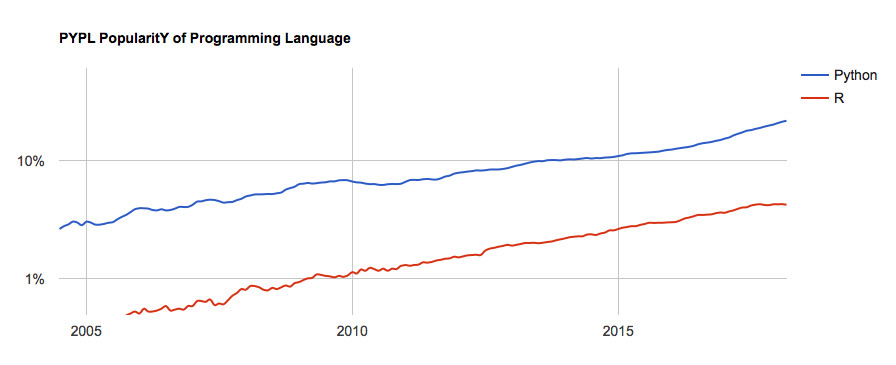
\includegraphics[scale=0.3]{fig/pypl}
\end{figure}


}



\frame{
\frametitle{Python for teaching Statistics}
\begin{center}
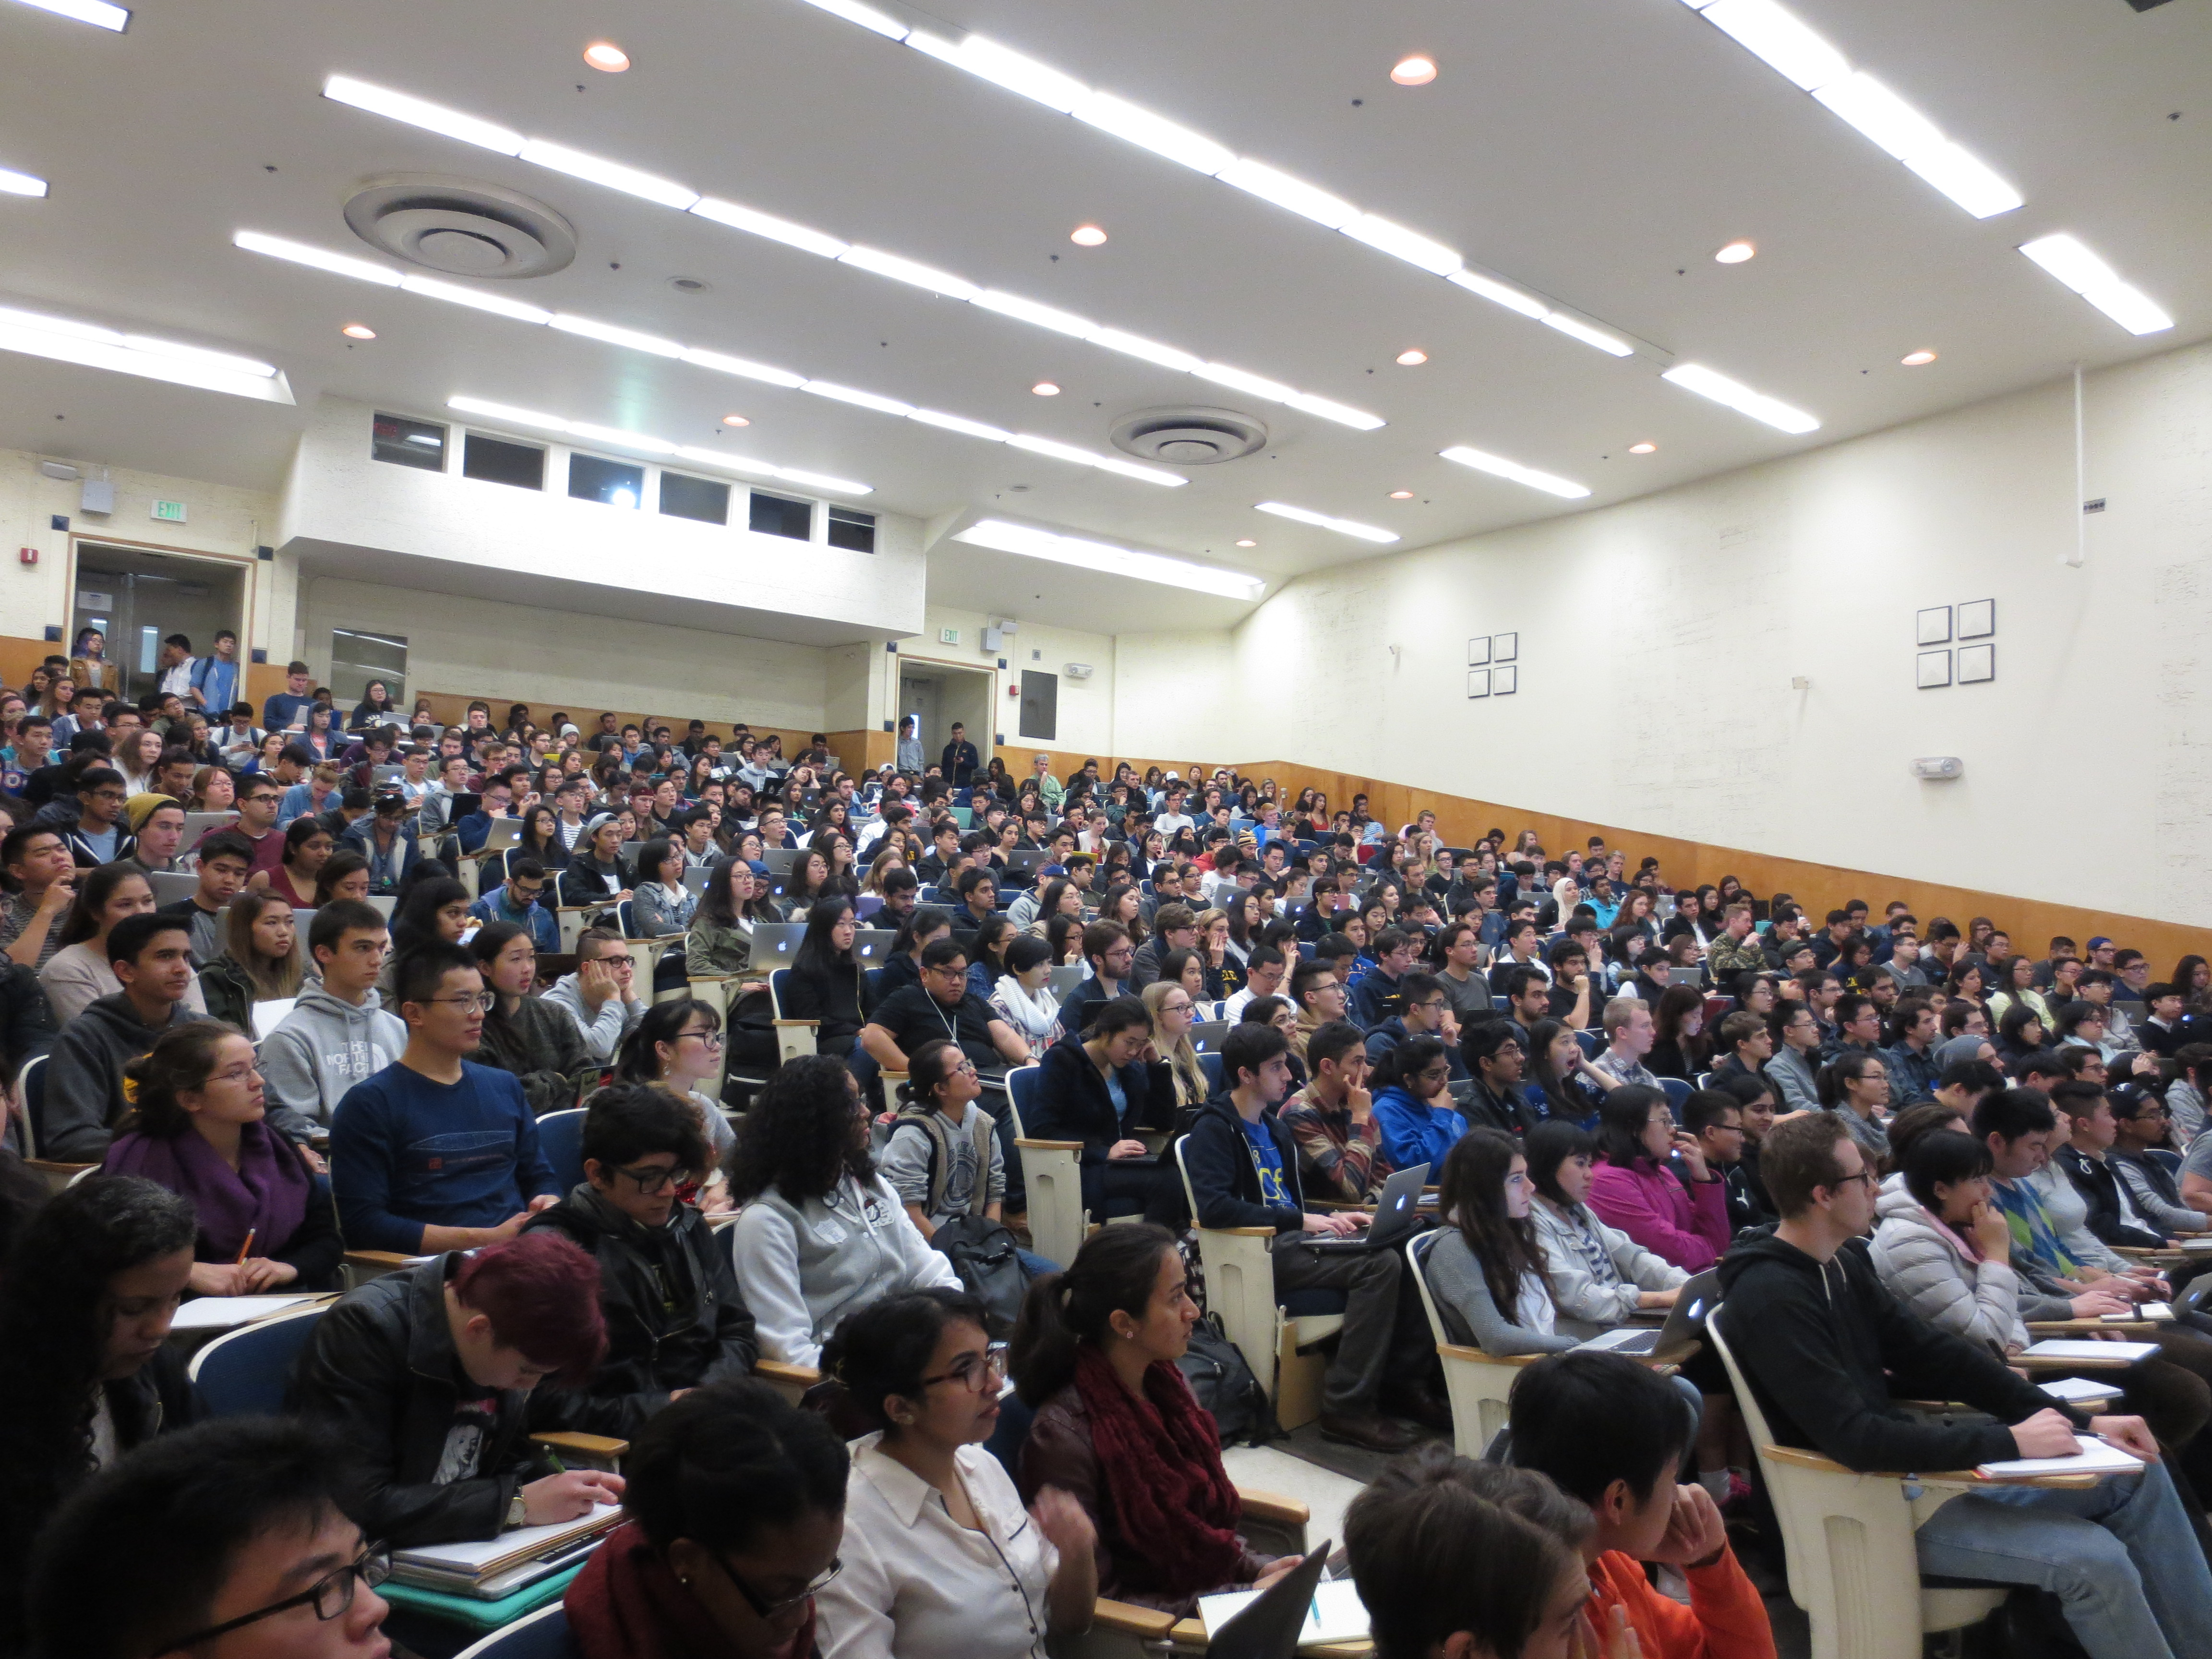
\includegraphics[width=0.9\textwidth]{fig/DS8.jpg} \\
Data Science 8, Spring 2016 at UC Berkeley
\end{center}
}




\section[Components of a Permutation Test]{Components of a Permutation Test}
\section[Randomized Experiments and Observational Studies]{Randomized Experiments and Observational Studies}

\frame
{
  \frametitle{Teaching Evaluations}
 \begin{center}
 \Large{ Student evaluations of teachers (SET) are used to} \\
  \begin{itemize}
  \item Quantify teaching effectiveness
  \item Compare instructors across courses
  \item Make hiring, firing, and promotion decisions  
  \end{itemize}
  \vfill
Are SET a valid measure of teaching effectiveness? 
\end{center}
}


\frame{
\frametitle{Teaching evaluations}
\large

In \citet{boring2016teaching}, we reanalyzed data from \cite{macnell2014whats}.
\vspace{10pt}
\begin{center}
\begin{itemize}
\itemsep 10pt
\item Students were randomized to 4 online sections of a course.
\item In two sections, the instructors swapped identities.
%\item Female-identified instructor was rated lower on average in all categories
\item Was the instructor who identified as female rated lower on average?
\end{itemize}
\end{center}
}


\frame{
\frametitle{Neyman-Rubin model, generalized}
Student $i$ is represented by a ticket with $4$ numbers, their response to each ``treatment.''

\begin{align*}
r_{ijk} &= \text{ SET given by student }i\text{ to instructor }j \\
&\text{ when they appear to have gender }k
\end{align*}
$$i = 1, \dots, N; \qquad j = 1,2; \qquad k \in \{ \text{male, female} \}$$

\vspace{10pt}
Numbers are fixed; randomization reveals one of the numbers. \\
\vspace{10pt}
Assume non-interference: each student's response depends only on that student's treatment. \\
\vspace{10pt}
If gender doesn't matter,
$$r_{ij\text{male}} = r_{ij\text{female}}.$$
}


\frame{
\frametitle{Randomization}

Conceptually, there are two levels of randomization:

\begin{enumerate}
\item $N_m$ students are randomly assigned to the male instructor, and
the remaining $N_f$ get the female instructor.
\item Of the $N_j$ assigned to instructor $j$, 
$N_{jm}$ are told that the instructor is male, for $j = 1, 2$.
\end{enumerate}
\vspace{10pt}

All ${{N_m}\choose{N_{mm}} }\times{ {N_f}\choose{N_{fm}}}$ assignments of students to sections
are equally likely. \\
\vspace{10pt}

\begin{block}{Stratified two-sample test}
\begin{itemize}
\item For each instructor, permute perceived gender assignments
\item Use difference in mean ratings for female-identified minus male-identified
\end{itemize}
\end{block}
}

\begin{frame}[fragile]
\frametitle{Code}
\begin{center}
\begin{python}
# load packages
import numpy as np
from permute.data import macnell2014
from permute.stratified import stratified_two_sample

# initialize PRNG
rs = np.random.RandomState(seed=1)

# load the data
ratings = macnell2014()

# Ratings vs reported instructor gender (difference in means)
(p, t) = stratified_two_sample(group=ratings.tagender,
                               response=ratings.overall,
                               condition=ratings.taidgender,
                               alternative="two-sided",
                               stat="mean", reps=10**5)
\end{python}
\end{center}
\end{frame}


\frame
{
  \frametitle{Results}
In all categories, the male-identified instructor was rated higher.
\begin{table}
\begin{tabular}{r|crr}
\textbf{Characteristic} & \textbf{M-F} & \textbf{perm} $P$ & \textbf{t-test} $P$ \\
\hline
Overall & 0.47 & 0.12 & 0.128\\
Caring & 0.52 & 0.10 & 0.071\\
Consistent & 0.47 & 0.21 & \textcolor{red}{0.045} \\ 
Enthusiastic & 0.57 & 0.06 & 0.112 \\
Fair & 0.76 & \textcolor{red}{0.01} & 0.188 \\
Feedback & 0.47 & 0.16 & 0.054 \\
Helpful & 0.46 & 0.17 & \textcolor{red}{0.049} \\
Knowledgeable & 0.35 & 0.29 & \textcolor{red}{0.038} \\
Praise & 0.67 & \textcolor{red}{0.01} & 0.153 \\
Professional & 0.61 & 0.07 & 0.124 \\
Prompt & 0.80 & \textcolor{red}{0.01} & 0.191 \\
Respectful & 0.61 & 0.06 & 0.124 \\
Responsive & 0.22 & 0.48 & \textcolor{red}{0.013}
\end{tabular}
\end{table}

}



\frame{
\frametitle{Omnibus Test}
\textbf{Nonparametric combination of tests (NPC):} combine individual p-values into a single omnibus test when there are many responses \\
\vspace{10pt}

Test whether to accept \textbf{all null} hypotheses or reject \textbf{at least one alternative} \\
\vspace{10pt}

\begin{block}{Fisher's combining function}
Let $\{ P_j\}_{j=1}^J$ be p-values for $J$ hypotheses. Define
$$X^2 = -2 \sum_{j=1}^J \ln(P_j)$$
If $\{ P_j\}_{j=1}^J$ are independent and all nulls are true, then $X^2 \sim \chi_{2J}^2$ . \\
\end{block}
}


\frame{
\frametitle{Omnibus Test}
Ratings by the same student for different categories are \textbf{dependent}.\\
\vspace{10pt}

$\implies$ Treat all ratings from a student as a vector and calibrate the distribution of $X^2$ using the this permutation distribution.
\vspace{10pt}

\begin{block}{NPC Permutation Procedure}
\begin{enumerate}
\item Calculate the vector of test statistics (use the \textbf{same permutation} of section memberships to compute all statistics), repeat a large number $B$ times
\item Compute the p-value for each individual variable in each permutation relative to the other values in the distribution
\item Apply the combining function to each vector of p-values.
\end{enumerate}
\end{block}
}



\begin{frame}[fragile]
\frametitle{Omnibus Test}
\begin{python}
# Initialize placeholders
ind = 0
test_distr = np.zeros( (10**5, len(categories)) )
pvalues = np.zeros( len(categories) )

# Loop over rating categories
for col in categories:
    (p, t, distr) = stratified_two_sample(
                        group=ratings.tagender,
                        response=ratings[col],
                        condition=ratings.taidgender,
                        alternative="two-sided",
                        stat="mean", seed = seed,
                        reps = 10**5, keep_dist = True)
    ind += 1
    test_distr[:,ind] = distr; pvalues[ind] = p
 
# NPC 
omnibus_pvalue = npc(pvalues, test_distr, combine="fisher", 
                         alternatives="two-sided")
\end{python}
\end{frame}

\frame{
\frametitle{Conclusions}
\large
\textbf{Omnibus test:} $P = 0$ \\
\vspace{20pt}

Reject the null hypothesis that there is no difference in ratings for any category. \\
\vspace{10pt}
$\implies$ SET measure something other than teaching effectiveness.
}




\section[Software and Statistics]{Algorithms and Pseudorandom Numbers}

\frame{
\frametitle{Download \texttt{permute}!}
\begin{figure}[htbp]
\begin{center}
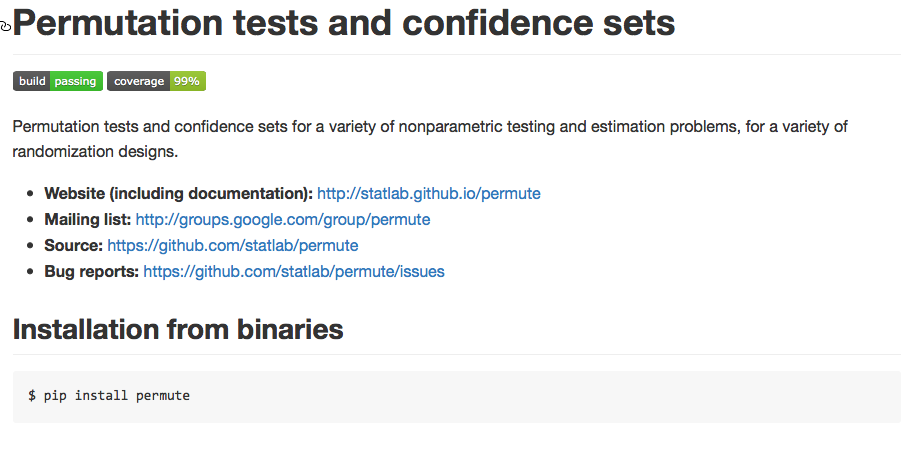
\includegraphics[width=\textwidth]{fig/github/permute}
\end{center}
\end{figure}


\url{https://github.com/statlab/permute}
}


\begin{frame}
\frametitle{References}
\tiny
\bibliographystyle{plainnat}
\bibliography{refs}
\itemize
\end{frame}


\end{document}
